\documentclass[10pt,journal,compsoc]{IEEEtran}
\usepackage{url}
\usepackage{booktabs}
\usepackage{threeparttable}
\usepackage{multirow}
\usepackage{amsthm,amsmath}
\usepackage{graphicx}
\usepackage{ragged2e}
\usepackage{fullpage}
\usepackage{float}
\usepackage[colorlinks,allcolors=black]{hyperref}
\usepackage[nocompress]{cite}
\renewcommand{\arraystretch}{1.05}

\begin{document}

	\title{MGRFE: multilayer recursive feature elimination based on an embedded genetic algorithm for cancer classification}

	\author{Cheng~Peng,
		Xinyu~Wu,
		Wen~Yuan,
		Xinran~Zhang,
		Yu~Zhang,
		and~Ying~Li
		\IEEEcompsocitemizethanks{\IEEEcompsocthanksitem C. Peng, X. Wu, W. Yuan, X. Zhang, Y. Zhang, and Y. Li are with the College of Computer Science and Technology, Key Laboratory of Symbol Computation and Knowledge Engineering of Ministry of Education, Jilin University, Changchun 130012, China.\protect\\

		\IEEEcompsocthanksitem Y. Li is the correspondence author. Email: liying@jlu.edu.cn.}
		\thanks{}}

	\markboth{Journal of \LaTeX\ Class Files,~Vol.~XX, No.~X, XXXX~2018}%
	{Peng \MakeLowercase{\textit{et al.}}: MGRFE: multilayer recursive feature elimination based on an embedded genetic algorithm for cancer classification}

	\IEEEtitleabstractindextext{
	\begin{abstract}
	\justifying
	Microarray gene expression data have become a topic of great interest for cancer classification and for further research in the field of bioinformatics. Nonetheless, due to the ``large \(p\), small \(n\)'' paradigm of limited biosamples and high-dimensional data, gene selection is becoming a demanding task, which is aimed at selecting a minimal number of discriminatory genes associated closely with a phenotype. Feature or gene selection is still a challenging problem owing to its nondeterministic polynomial time complexity and thus most of the existing feature selection algorithms utilize heuristic rules.
	A multilayer recursive feature elimination method based on an embedded integer-coded genetic algorithm with a dynamic-length chromosome, MGRFE, is proposed here, which is aimed at selecting the gene combination with minimal size and maximal information. On the basis of 19 benchmark microarray datasets including multiclass and imbalanced datasets, MGRFE outperforms state-of-the-art feature selection algorithms with better cancer classification accuracy and a smaller selected gene number. MGRFE could be regarded as a promising feature selection method for high-dimensional datasets especially gene expression data. Moreover, the genes selected by MGRFE have significant biological relevance to cancer phenotypes. The source code of our proposed algorithm and all the 19 datasets used in this paper are available at \url{https://github.com/Pengeace/MGRFE-GaRFE}.
	\end{abstract}
		
	\begin{IEEEkeywords}
	Gene selection, Genetic algorithm, Recursive feature elimination, Microarray data, Cancer classification.
	\end{IEEEkeywords}}
	
	\maketitle
	\IEEEpeerreviewmaketitle
	
	\IEEEraisesectionheading{\section{Introduction}}

	\IEEEPARstart{O}{ne} chief challenge in bioinformatics is the ``large \(p\) small \(n\)'' paradigm \cite{W1}, on account of ever-increasing high-dimensional data and limited available experimental samples. In particular, for gene expression data, the sample number is distinctively small compared with several thousand to tens of thousands of genes. 
	For the analysis of high-dimensional data, feature selection is essential, which is designed to remove irrelevant and redundant features, thus cutting down the dimensionality and improving the predictive performance and model interpretability. On the other hand, due to its nondeterministic polynomial (NP) time complexity, feature selection is still a challenging and extensively studied problem in the machine learning and data mining fields. 
	As for the field of bioinformatics, there are numerous high-dimensional biological data in sequence analysis, microarray analysis, and spectral analysis. This situation makes feature selection more important and challenging.
	On the basis of the process of choosing features for classification, feature selection methods can be roughly subdivided into three categories: filter, wrapper, and hybrid techniques \cite{W6}.
	
	Filter algorithms generally evaluate features according to the inherent characteristic of a dataset, then rank all the features and preserve only an optimal subset of the original features. Up to now, lots of filter algorithms have been designed, such as the methods based on the \textit{t}-test \cite{W23}, $\chi^2$ test \cite{W21}, mutual information \cite{W22}, maximal information coefficient (MIC) \cite{W25}, and signal-to-noise ratio \cite{W24}. The \textit{t}-test is the frequently used and efficient statistical approach to detecting differentially expressed genes in microarray analysis \cite{RN413, RN414, RN421, RN417, RN418, RN419, RN416}. MIC is an information theory-based measurement for capturing a wide range of associations, which has shown excellent performance on detecting novel associations in large datasets \cite{W8}. The recent study of McTwo \cite{W16}, which is based on MIC for selection of a gene subset in a microarray data, has outperformed most of existing algorithms. In addition, MIC may offer more convenience in dealing with multiclass datasets. Hence, the \textit{t}-test and MIC are practicable and qualified approaches for selecting statistically significant discriminative genes and thus are mostly used in the feature preprocessing stage to generate a candidate gene set in the analysis of microarray. Because there is no classification algorithm involved in the filter algorithm, its computational speed is high and suitable for large datasets. On the other hand, the filter techniques for gene feature selection also have some limitations. First, filter methods are likely to add redundant features into the chosen subsets, which will lead to inaccessibility of optimal results. Second, genes in the cell interact with other genes to perform a certain biological function, but the filter methods select genes individually rather than gene combinations \cite{P34}. Third, the features top-ranked by a filter algorithm are not always the best features for classification \cite{W16}.
	
	Wrapper algorithms usually employ classification models and contain heuristic rules to select feature subsets guided by the classification performance on the feature subsets being used, which are usually superior to filter algorithms but more time-consuming. A variety of wrapper algorithms have emerged involving simulated annealing, randomized hill climbing \cite{W26}, regularized random forest (RRF) \cite{W11}, particle swarm optimization (PSO) \cite{W12,W10}, and genetic algorithm (GA) \cite{W13}. With the rapid development of heuristic rules and evolutionary strategies commonly present in wrapper techniques, various swarm intelligence algorithms have been applied to the optimization of feature selection. Kar \emph{et~al.} have proposed a particle swarm optimization method based on adaptive K-nearest neighborhood (KNN) to identify a minimum meaningful gene subset \cite{W15}. Moosa \emph{et~al.} have presented a modified artificial bee colony algorithm (ABC) to select a minimum number of genes with high predictive accuracy for cancer classification \cite{P32}. Oreski \emph{et~al.} have designed a hybrid GA with neural networks to identify an optimal feature subset with high classification accuracy and scalability for credit risk assessment \cite{W17}. Jung and Zscheischler have described a guided hybrid GA to minimize the number of cost function evaluations \cite{W18}. Nevertheless, all these feature selection methods based on swarm intelligence algorithms use the binary encoding method and lack an explicit reduction in the feature number. The feature number only changes in the randomized evolution operation like mutation and crossover. Thus, these methods lack the precise control over the gene features in the individuals and can not explicitly remove genes to decrease the feature number. Meanwhile, it has been verified that only a minimal number of informative genes is enough for effective diagnosis of different phenotypes in microarray gene datasets \cite{P1,W16,P32,P33}. The feature selection using binary encoding has three main shortcomings in finding an optimal gene combination: (1) The fixed chromosome length for the encoding length must be equal to the gene range to represent all the genes. This arrangement can result in impossibility of the explicit reduction in the gene number and unnecessary space occupation when there are only several 1s among lots of 0s. (2) There are different numbers of actual existing genes in different individuals. Because there are different numbers of 1s, the actual number of genes varies among individuals and cannot be controlled precisely. (3) The convergence speed is usually low and the time cost is high to generate the minimal informative gene combination. 
	The sizes of the optimal gene combinations in most of datasets are below 10. The evolution-based feature selection algorithms using binary encoding lack of an explicit feature reduction mechanism, which results in low probability and high time cost to generate the optimal minimal gene combination among the several thousand to tens of thousands of genes in each dataset.
	Recursive feature elimination (RFE) is a popular strategy that yields an explicit recursive feature reduction by removing features with the least weights \cite{W7,P1,P2,P27}.
	
	Hybrid algorithms are the combination of filter and wrapper strategies \cite{W6}. First, the filter algorithms are applied to remove irrelevant features and narrow the search space. Second, the wrapper algorithms are performed on the pre-selected subsets to accomplish optimal feature selection. Hybrid algorithms can take advantage of both filter and wrapper techniques.
	
	A multilayer recursive feature elimination method with an embedded integer-coded genetic algorithm, MGRFE, is proposed here, which can be categorized into a hybrid algorithm. On the one hand, MGRFE uses the \textit{t}-test and MIC in the search space reduction stage to generate a candidate gene set. On the other hand, MGRFE combines the advantages of both evolution calculation of GA and the explicit feature elimination of RFE to achieve the minimum discriminative gene subset with optimal classification ability.
	To validate the performance of the proposed method, we comprehensively compared our proposed MGRFE with the feature selection methods from 20 representative studies on 19 benchmark gene expression datasets including multiclass and imbalanced datasets. The comparison results show that our method outperforms most of state-of-the-art feature selection algorithms. MGRFE can select a smaller gene subset but yield the same or higher classification accuracy than other algorithms. Furthermore, the specific biomedical relevance of the selected genes to the related cancer phenotypes has also been verified by text mining. The whole work flow of this study is presented in Fig. \ref{Fig:MGRFE_whole}.

	
	\begin{figure*}[!htbp]
		\centering
		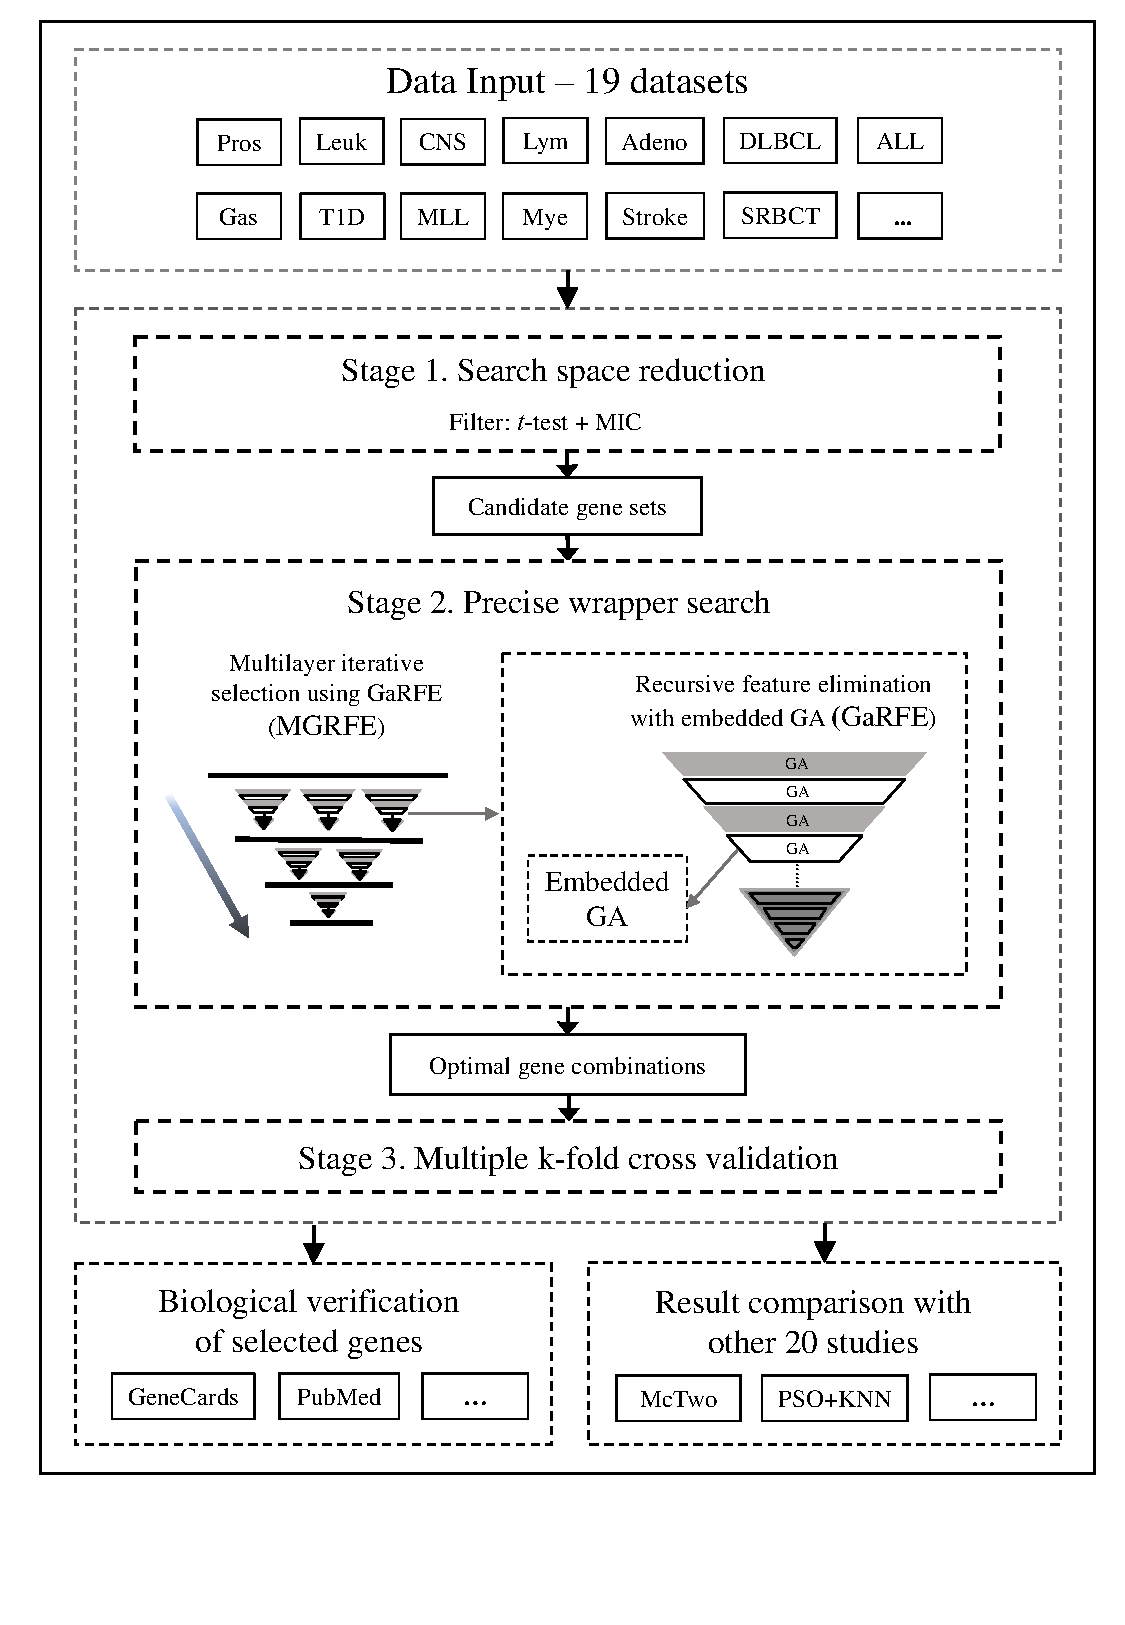
\includegraphics[width=0.6\textwidth]{pictures/MGRFE-whole.pdf}
		\caption{A flowchart of the whole MGRFE procedure in this study.}
		\label{Fig:MGRFE_whole}
	\end{figure*}
	
	\section{Materials and Methods}
	\subsection{Materials}
	
	This study involves 19 benchmark microarrays including binary, multiclass, balanced, and imbalanced datasets, which are subdivided into two large datasets.
	Dataset One consists of the 17 binary classification datasets used in ref. \cite{W16}, which includes diffuse large B-cell lymphoma (DLBCL) \cite{Y22}, Prostate (Pros) \cite{Y23}, acute lymphoblastic leukemia (ALL; subdivided into four subtypes based on different phenotypes) \cite{Y24}, central nervous system embryonal tumor (CNS) \cite{Y25}, Lymphoma (Lym) \cite{Y26}, Adenoma (Adeno) \cite{Y27}, Colon \cite{Y20}, Leukaemia (Leuk) \cite{Y21}, Myeloma (Mye)\cite{Y28}, Gastric (Gas) \cite{Y29}, and Gastric1/Gastric2 (Gas1/Gas2) cancer \cite{Y30} as well as type 1 diabetes (T1D) \cite{Y31}, and Stroke \cite{Y32}. Among them, DLBCL, Colon, Leukaemia, Myeloma, ALL1-4, and CNS datasets are imbalanced.
	Dataset Two is composed of the three typical benchmark microarray datasets used in ref. \cite{W15}, including two multiclass datasets of small-round blue-cell tumor (SRBCT) \cite{P13} and mixed lineage leukemia (MLL) \cite{W3} and one binary dataset of acute lymphoblastic leukemia and acute myeloid (ALL\_AML). Many previous experiments are conducted on these three datasets \cite{P8,P9,P10,P11,P12,P13,P14,P15,P16,P17,P18,P19,P20,P21,P22,P23}. The performance comparison between these methods and MGRFE will be provided in the Results section. It should be mentioned that the widely used benchmark Leukaemia was tested in both refs. \cite{W16} and \cite{W15} named as Leuk and ALL\_AML respectively, but they are same actually.
	The information on the 19 datasets in the two large datasets is given in Tables 1 and 2 in Supplementary Material. All these datasets can be downloaded directly from \url{https://github.com/Pengeace/MGRFE-GaRFE}.
	
	\subsection{Classification performance measurements}
	
	On the 17 binary classification datasets, we performed six widely used measurements to compare the performance: Accuracy ($Acc$), Sensitivity ($Sn$), Specificity ($Sp$), Average accuracy ($Avc$), Matthews Correlation Coefficient($MCC$), and $AUC$. $AUC$ is the area under the receiver operating characteristic (ROC) curve, and the formulas of the other five measurements are presented in Equation (\ref{eq:1}). In Equation (\ref{eq:1}), $P$ and $N$ represent the numbers of positive and negative samples; $TP$ and $TN$ mean the number of correctly predicted positive and negative samples; and $FP$ and $FN$ denote the wrongly predicted positive and negative samples, respectively. For the two multiclass datasets, for consistency and convenience, only \(Acc\) is used.
	
	{\scriptsize
		\begin{equation}\label{eq:1}
		\begin{split}
		Sn = & \frac{TP}{TP+FN} ,\quad Sp = \frac{TN}{TN+FP}, \\
		Acc = & \frac{TP+TN}{P+N} ,\quad Avc = \frac{Sn+Sp}{2}, \\
		MCC = & \frac{TP \cdot TN-FP \cdot FN}{\sqrt{(TP+FP)(TP+FN)(TN+FP)(TN+FN)}}\\
		\end{split}
		\end{equation}
	}
	
	\subsection{Method}
	
	As shown in Fig. \ref {Fig:MGRFE_flowchart}, the proposed MGRFE is divided into three stages, which are (1) Search space reduction; (2) Precise wrapper search and (3) Multiple k-fold cross-validation (CV). MGRFE is a multilayer iterative feature selection method with GaRFE acting as the feature selection unit in every layer. GaRFE is a recursive feature elimination process including embedded GA. The Pseudocodes 1, 2 and 3 in Supplementary Material provide the pseudocodes of the processes MGRFE, GaRFE and embedded GA.
	
	\begin{figure*}[t]
		\centering
		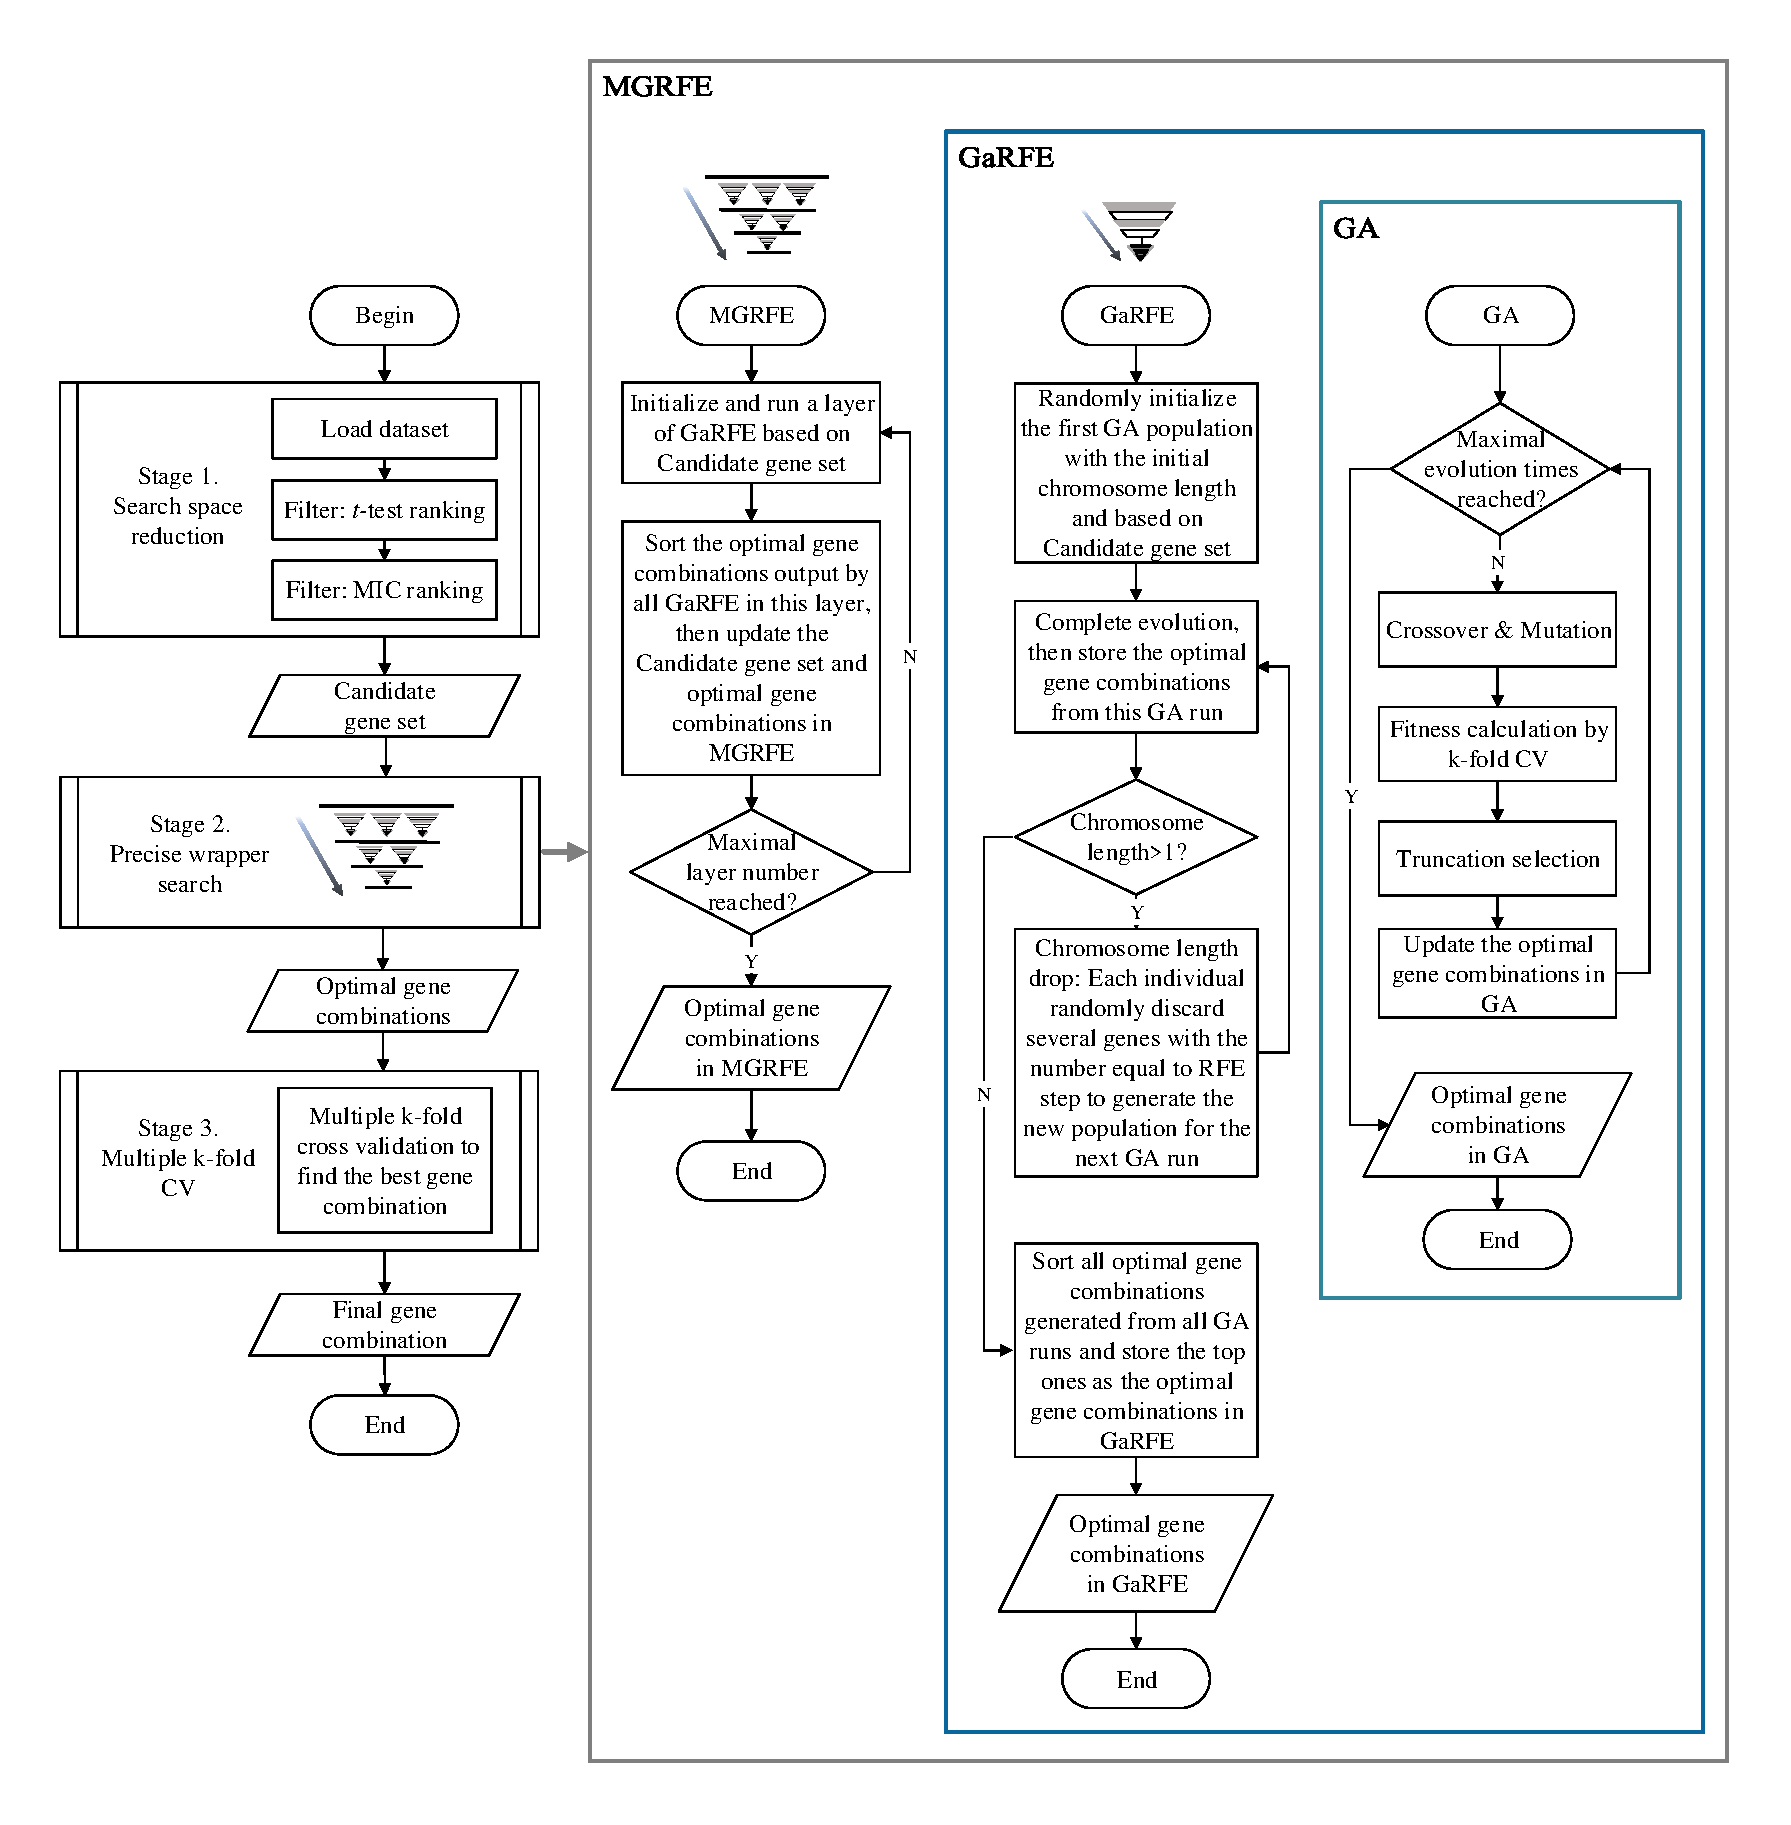
\includegraphics[width=0.87\textwidth]{pictures/MGRFE-flowchart.pdf}
		\caption{The flowchart of MGRFE, which is divided into 3 stages: search space reduction, precise wrapper search, and multiple k-fold CV. Stage 2 is the core of MGRFE, which includes two key processes: GaRFE and embedded modified GA.}
		\label{Fig:MGRFE_flowchart}
	\end{figure*}
	
	\subsubsection{Stage 1: Search space reduction}
	
	At Stage 1, two filter methods, the \textit{t}-test and MIC, are used to decrease the gene range and offer a candidate gene set for later precise wrapper search stage. First, we perform the \textit{t}-test on all genes and subject them to ascending sorting according to their $p$ values, then the top-ranked statistically significant features with $p$ values less than 0.05 are preserved. Next, the upper limit of the features kept after the \textit{t}-test is set to 1000, that is, when there are more than 1000 features having $p$ values less than 0.05, only the top 1000 with lower $p$ values would be kept. If the preserved features after the \textit{t}-test screening are fewer than 500, they are all kept directly and definitively to form the candidate gene set without MIC screening; otherwise, the MIC-based selection will be followed. Second, we carry out MIC calculation on the preserved genes and resort them according to their MIC values, then the candidate gene set is generated from the top 500 genes with higher MIC values. For the two multiclass datasets, a candidate gene set is generated based only on the descending order of MIC values of all genes for which the multivariate \textit{t}-test cannot be performed directly. 
	In the Table 5 in Supplementary Material, the number of statistically significant genes with \emph{t}-test-based \emph{p}-values less than 0.05 on each binary-class dataset are listed.
	In the "S8" section of Supplementary Material, we also give a simple comparison of \textit{t}-test+MIC with other filter combinations.

	\subsubsection{Stage 2: Precise wrapper search}
	
	At Stage 2, we search the candidate gene set obtained from Stage 1 and compute the optimal gene combinations for further selection at Stage 3. MGRFE is a multilayer iterative feature selection method and its selection unit in each layer is a GaRFE process. GaRFE, the inverted triangle in MGRFE as shown in Fig. \ref{Fig:MGRFE_whole}, is the recursive feature elimination process with every stair being embedded GA. Embedded GA is the integer-coded genetic algorithm with a dynamic-length chromosome. The key feature of MGRFE is GaRFE in each layer, in which embedded GA is responsible for generating optimal gene combinations, and the RFE process is responsible for cutting down the gene number. Therefore, our method can find gene combinations with both significantly reduced sizes and excellent classification performance.
	
	\noindent\textbf{Embedded GA:}
	
	In our method, the modified GA using variable-length integer-coded chromosome is embedded in the RFE process as each stair in the inverted triangle of GaRFE. The embedded GA includes the following steps. First, we initialize the GA population by a certain amount of individuals representing gene combinations with the same sizes. Then, we perform fitness calculation and genetic operators including mutation, crossover, and selection until the stopping criterion is satisfied. In the end, we return the best individuals that represent the best gene combinations to GaRFE. The stopping criterion of embedded GA is iteration time, which is set to 1 to 3.
	
	To embed GA in the RFE process and achieve the minimal informative genes, some modifications are made in the original GA. The embedded GA uses variable-length integer-coding technique for the chromosome in a GA individual, and each individual has a set of integers representing different genes to make up a gene combination. In every run of GA, the gene combinations represented by different individuals all have a fixed size. Between two adjacent GA runs in the RFE process, every individual sheds the same number of genes from its chromosome.
	
	A truncation selection method is used as the selection operator in embedded GA \cite{P37}, which simply ranks all individuals and selects the top ones to form the next generation. The mutation and crossover operators for generating new individuals are adjusted to adapt to the variable-length integer-encoding technique. One main challenge that should be addressed in these two processes is avoidance of duplicated genes in every individual, which leads to the decline of the number of actual existing genes. Based on our encoding technique, the mutation operation for an individual is randomly changing some genes to others. It should be ensured that new genes do not exist in this individual previously to avoid repetitions. Crossover in embedded GA also involves single-point crossover which is the most widely used crossover method in binary encoding. Specifically, a random position is selected in the chromosome, and two parent individuals split themselves at this crossover point and then exchange chromosome tails to generate children individuals. After the crossover, the potential duplicate genes in the children individuals are replaced with other genes from their parents to avoid decreasing the gene number. Fitness (\(F\)) of an individual is defined in Equation (\ref{eq:2}):
	{
		\scriptsize
		\begin{eqnarray}\label{eq:2}
		F = \left\{
		\begin{array}{cl}
		Acc & {,{balanced\ dataset}}\\
		\alpha Acc + (1-\alpha)Avc & {,{imbalanced\ dataset}}\\
		\end{array} \right.
		\end{eqnarray}
	}
	, where \(\alpha\) is an adjustment coefficient to deal with the imbalanced datasets. For imbalanced datasets, fitness defined as \(\alpha Acc +(1-\alpha)Avc\) can adjust the trend of predicting samples as abundant classes for \(Avc = (Sn + Sp) \big/ 2\) takes the correct prediction proportion of both sample classes into consideration. In our experiments, we take \(\alpha\) 0.6 for imbalanced datasets. For balanced datasets, \(F\) is simply defined as \(Acc\). \(F\) is calculated by 5-fold CV, and the employed classifier is Naive Bayes classifier (NBayes) \cite{P35}. We sort different GA individuals based on two metrics, \(F\) and gene number. The individual with higher \(F\) is superior. For two individuals with the same \(F\) values, the one with a smaller gene number is superior. MGRFE and GaRFE also use the above-mentioned sorting rule to rank different gene combinations.
	
	\noindent\textbf{Recursive feature elimination with embedded GA:}
	
	GaRFE as shown in Fig. \ref {Fig:MGRFE_flowchart} is designed as an explicit recursive feature elimination process with embedded GA to find minimal discriminatory gene combinations. First, we randomly generate the initial GA population based on a certain candidate gene set and chromosome length. Then, we implement a chromosome length drop and a GA run in turns until the chromosome length in GA drops to 1. Finally, we sort the optimal gene combinations from all GA runs and then return the overall top-ranked gene combinations to MGRFE. The chromosome length drop means that every individual in the current GA population randomly discards the same number of genes to generate the new GA population for the next run. The number of discarded genes between two GA runs, the RFE step, is set from 1 to 3 according to the current chromosome length. A larger decline step is set for larger chromosome length to avoid time cost and a smaller decline step set for smaller chromosome length to do precise searching.
	
	\noindent\textbf{Multilayer iterative selection:}
	
	MGRFE is designed as a multilayer iterative feature selection method with the selection unit in each layer being GaRFE. In every iteration layer, the GaRFE processes analyze the current candidate gene set and return their obtained optimal gene combinations. Then the candidate gene set is reduced and subjected to the next layer of iterative selection. The candidate gene set used by the first layer of MGRFE is from the search space reduction stage. After each iteration layer, all optimal gene combinations in MGRFE will be sorted and the top-ranked ones will form the updated reduced candidate gene set. After the specified layers of iteration, MGRFE sorts all the optimal gene combinations and provides the top-ranked gene combinations for Stage 3 to execute further validation.
	
	\subsubsection{Stage 3: Multiple k-fold CV to select the final gene combination}
	
	Stage 3 is aimed at finding the optimal gene combination with the best classification performance and minimal variance among different CV processes. K-fold CV is used for calculating the fitness of a GA individual. Multiple k-fold CV based on different random seeds is performed to further validate and select the final optimal gene combination.
	
	\section{Results}
	
	In this section, our proposed MGRFE is comprehensively compared with the state-of-the-art algorithms of gene selection on 19 benchmark datasets.
	Additionally, the biological verification of the selected genes is discussed.
	
	\subsection{Results on Dataset One}
	 
	The results of MGRFE on Dataset One including 17 binary datasets are given in Table \ref{Tab:RST all index}, where six measurements calculated by 5-fold CV and the \textit{t}-test and MIC-based gene rankings are listed. For 17 datasets, \(Acc\) values are all above 0.9 within 10 genes. Moreover, for 8 of 17 datasets (DLBCL, Leuk, ALL1, Lym, Adeno, Gas, Gas2, and Stroke), \(Acc\) reached 1.0 with gene number less than 5. MGRFE also show the strong robustness in dealing with imbalanced datasets like DLBCL, Colon, Leuk, ALL1, ALL4, and CNS, for which \(Sn\), \(Sp\), \(Avc\), \(MCC\), and \(AUC\) are all above 0.95 without being influenced by the data imbalance. 
	According to the \textit{t}-test and MIC-based gene ranking, the best gene feature subset is not always the highest-ranked features in the filter method, thus the filter algorithm alone cannot generate the optimal feature combination.
	It could be noted that the relative positions of selected genes in the two ranking methods are consistent on most datasets. The top-ranked genes in the \textit{t}-test are also top-ranked in the MIC sorting (e.g. the selected gene on ALL1 is the top one in both \textit{t}-test and MIC ranking). For 5 of 17 datasets, the top one gene  according to the \textit{t}-test appeared in the final selected gene subsets. Generally, the selected informative genes are top-ranked by the \textit{t}-test and MIC methods. Therefore, the filter techniques are qualified for the search space reduction stage. Moreover, MGRFE achieves stable classification performance in 10 repetitions of 10-fold CV as depicted in Fig. \ref{Fig:CV1}. Besides, we also validated the selected gene features of Leuk, Gas1 and Gas2 on independent datasets in the "S8" section of Supplementary Material.
	
	\begin{table*}[!htbp] \footnotesize
		\centering
		\caption{Results of MGRFE on 17 datasets in Dataset One}
		\label{Tab:RST all index}
		\resizebox{0.95\textwidth}{!}{
			\begin{tabular}{l|lllllllll}
				\toprule
				Datasets & Pos/Neg & Genes/Total & $Sn$ & $Sp$ & $Acc$ & $Avc$ & $MCC$ & $AUC$ & \textit{t}-test/MIC-based gene rankings\\
				\midrule
				DLBCL & 58/19 & \textbf{3}/7129 & 1.0 & 1.0 & \textbf{1.0} & 1.0 & 1.0 & 1.0 & [13/8, 39/24, 54/52]\\
				Pros & 52/50 & \textbf{4}/12625 & 0.980 & 0.982 & \textbf{0.981} & 0.981 & 0.963 & 0.98 & [1/1, 15/47, 74/49, 694/618]\\
				Colon & 40/22 & \textbf{6}/2000 & 1.0 & 0.960 & \textbf{0.985} & 0.980 & 0.969 & 0.97 & [15/6, 58/21, 176/297, 225/80, 240/555, 495/482]\\
				Leuk & 47/25 & \textbf{2}/7129 & 1.0 & 1.0 & \textbf{1.0} & 1.0 & 1.0 & 1.0 & [4/3, 7/5]\\
				Mye & 137/36 & \textbf{7}/12625 & 0.963 & 0.839 & \textbf{0.937} & 0.901 & 0.816 & 0.95 & [3/3, 15/103, 83/142, 143/13, 378/217, 404/644, 569/707]\\
				ALL1 & 95/33 & \textbf{1}/12625 & 1.0 & 1.0 & \textbf{1.0} & 1.0 & 1.0 & 1.0 & [1/1]\\
				ALL2 & 65/35 & \textbf{8}/12625 & 0.914 & 0.908 & \textbf{0.910} & 0.911 & 0.829 & 0.94 & [1/80, 52/395, 78/3040, 80/1297, 522/2448, 687/2038, 737/920, 760/1449]\\
				ALL3 & 24/101 & \textbf{8}/12625 & 0.830 & 0.950 & \textbf{0.927} & 0.890 & 0.785 & 0.93 & [4/500, 52/3437, 75/3010, 142/393, 488/443, 510/795, 715/1551, 770/1321]\\
				ALL4 & 26/67 & \textbf{6}/12625 & 1.0 & 0.986 & \textbf{0.990} & 0.993 & 0.978 & 0.99 & [1/2, 6/45, 39/356, 282/226, 535/497, 754/1377]\\
				CNS & 39/21 & \textbf{7}/7129 & 1.0 & 1.0 & \textbf{1.0} & 1.0 & 1.0 & 0.98 & [9/907, 53/542, 130/620, 131/519, 272/57, 273/454, 520/49]\\
				Lym & 22/23 & \textbf{3}/4026 & 1.0 & 1.0 & \textbf{1.0} & 1.0 & 1.0 & 1.0 & [4/7, 5/4, 669/135]\\
				Adeno & 18/18 & \textbf{1}/7457 & 1.0 & 1.0 & \textbf{1.0} & 1.0 & 1.0 & 1.0 & [468/27]\\
				Gas & 29/36 & \textbf{3}/22645 & 1.0 & 1.0 & \textbf{1.0} & 1.0 & 1.0 & 1.0 & [22/1, 77/32, 306/36]\\
				Gas1 & 72/72 & \textbf{3}/22283 & 0.986 & 0.973 & \textbf{0.980} & 0.980 & 0.961 & 0.99 & [132/74, 248/167, 717/500]\\
				Gas2 & 62/62 & \textbf{2}/22283 & 1.0 & 1.0 & \textbf{1.0} & 1.0 & 1.0 & 1.0 & [38/6, 89/62]\\
				T1D & 57/44 & \textbf{7}/54675 & 0.911 & 0.912 & \textbf{0.911} & 0.912 & 0.826 & 0.94 & [14/2229, 25/1579, 113/1287, 559/1282, 578/353, 680/426, 978/1728]\\
				Stroke & 20/20 & \textbf{4}/54675 & 1.0 & 1.0 & \textbf{1.0} & 1.0 & 1.0 & 1.0 & [1/3, 23/115, 129/543, 276/539]\\
				\bottomrule
		\end{tabular}}
	\end{table*}
	\begin{figure*}[htbp]
		\centering
		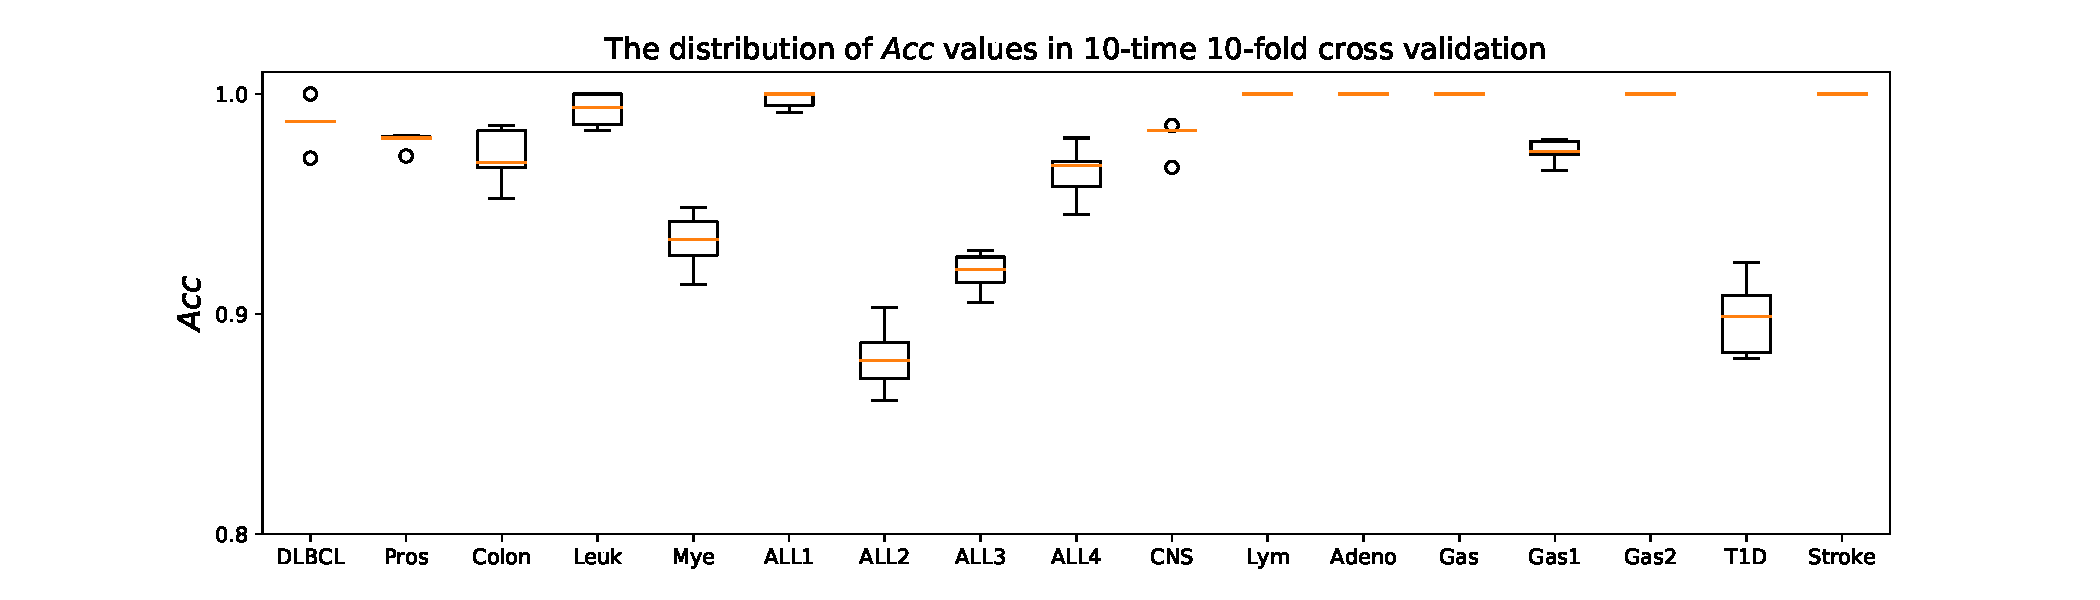
\includegraphics[width=0.72\textwidth]{pictures/CV1.pdf}
		\caption{The distribution of $Acc$ values in 10-time 10-fold CV for the selected gene combinations of 17 datasets in Dataset One.}
		\label{Fig:CV1}
	\end{figure*}
	
	\subsection{Comparison with other methods on Dataset One}
	
	McTwo \cite{W16} thoroughly tested all the datasets in Dataset One and demonstrated satisfactory performance. Here, we present the performance comparison between McTwo and MGRFE. Table \ref{Tab:CMP McTwo RST} lists the overall maximal \(Acc\) and numbers of selected genes on total 17 datasets for MGRFE and McTwo. For a more intuitive comparison, Fig. \ref{Fig:CMP McTwo} offers the line chart of maximal \(Acc\) achieved by the two algorithms on 17 datasets, where MGRFE obviously outperforms McTwo with a higher \(Acc\) line. On five datasets ALL2, ALL3, ALL4, Stroke and CNS, MGRFE achieves distinctly better classification performance than McTwo with relatively more genes. For a fairer and more specific comparison, the \(Acc\) values of the two algorithms are listed when the gene number of MGRFE is equal to McTwo as shown in Table \ref{Tab:same gene num}. The results indicate that MGRFE still outperforms McTwo. Nonetheless, the \(Acc\) values associated with the usage of the gene numbers fall behind our optimal \(Acc\) values on these datasets obviously. Thus, MGRFE selected somewhat more genes to achieve the optimal results.
	
	\begin{figure*}[ht]
		\centering
		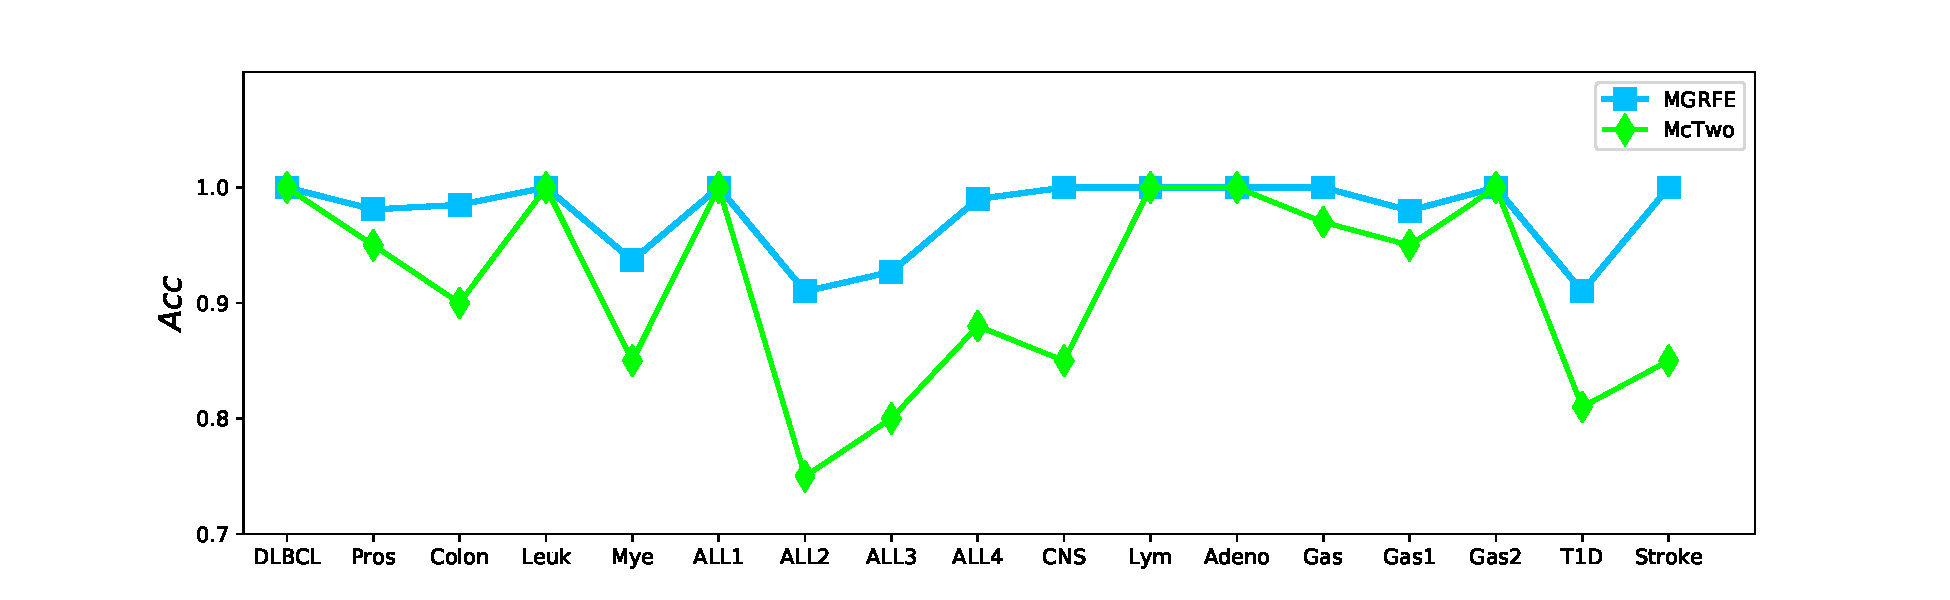
\includegraphics[width=0.72\textwidth]{pictures/CMP-McTwo.pdf}
		\caption{The line plots of overall maximal accuracy for MGRFE and McTwo on 17 datasets in Dataset One.}
		\label{Fig:CMP McTwo}
	\end{figure*}
	
	\begin{table*}[t]
		\centering
		\caption{Performance comparison between McTwo and MGRFE on 17 datasets in Dataset One}
		\label{Tab:CMP McTwo RST}
		\resizebox{1.0\textwidth}{!}{
			\begin{tabular}{llllllllllllllllll}
				\toprule
				& DLBCL & Pros & Colon & Leuk & Mye & ALL1 & ALL2 & ALL3 & ALL4 & CNS & Lym & Adeno & Gas & Gas1 & Gas2 & T1D & Stroke\\
				\midrule
				MGRFE \(Acc\) & 1.0 & 0.981 & 0.985 & 1.0 & 0.937 & 1.0 & 0.910 & 0.927 & 0.990 & 1.0 & 1.0 & 1.0 & 1.0 & 0.980 & 1.0 & 0.911 & 1.0\\
				McTwo \(Acc\) & 1.0 & 0.95 & 0.9 & 1.0 & 0.85 & 1.0 & 0.75 & 0.8 & 0.88 & 0.85 & 1.0 & 1.0 & 0.97 & 0.95 & 1.0 & 0.81 & 0.85\\
				MGRFE Genes & 3 & 4 & 6 & 2 & 7 & 1 & 8 & 8 & 6 & 7 & 3 & 1 & 3 & 3 & 2 & 7 & 4\\
				McTwo Genes & 4 & 3 & 6 & 2 & 7 & 1 & 2 & 5 & 2 & 4 & 4 & 2 & 3 & 4 & 2 & 6 & 1\\
				\bottomrule
		\end{tabular}}
	\end{table*}
	
	\begin{table}[htbp] \scriptsize
		\centering
		\caption{Performance comparison on five datasets between MGRFE and McTwo when MGRFE uses the same gene numbers as McTwo does}
		\label{Tab:same gene num}
		\begin{tabular}{llll}
			\toprule
			Datasets & Methods & Genes & $Acc$\\
			\midrule
			ALL2 & MGRFE & 2 & 0.760\\
			& McTwo & 2 & 0.75\\\hline
			ALL3 & MGRFE & 5 & 0.874\\
			& McTwo & 5 & 0.8\\\hline
			ALL4 & MGRFE & 2 & 0.896\\
			& McTwo & 2 & 0.88\\\hline
			CNS & MGRFE & 4 & 0.921\\
			& McTwo & 4 & 0.85\\\hline
			Stroke & MGRFE & 1 & 0.825\\
			& McTwo & 1 & 0.75\\
			\bottomrule
		\end{tabular}
	\end{table}
	\subsection{Results on Dataset Two}
	
	Here we present the results of MGRFE on Dataset Two including three benchmark datasets, where two datasets are multiclass datasets. MGRFE selects five, two, and three genes in SRBCT, ALL\_AML, and MLL respectively and the overall maximal \(Acc\)s are all 1.0 in 5-fold CV. Fig. \ref{Fig:3 RFE on benchmarks} offers three instances of GaRFE processes in the first layer of MGRFE for these datasets, where we can notice that the \(Acc\) values of the best GA individuals are kept at 1.0 in the majority of gene number ranges and begin to drop only when the gene number is significantly reduced. We also carried out 10 repetitions of 10-fold CV to further validate the final selected gene combinations in Dataset Two as shown in Fig. \ref{Fig:CV2}. The mean of \(Acc\)s for SRBCT, ALL\_AML, and MLL are 1.0, 0.982, and 0.997, respectively, with standard deviations being 0.0, 0.008, and 0.006. These data confirm that MGRFE has high classification stability.
	
	\begin{figure*}[!htbp]
		\begin{minipage}[t]{0.3\textwidth}
			\centering
			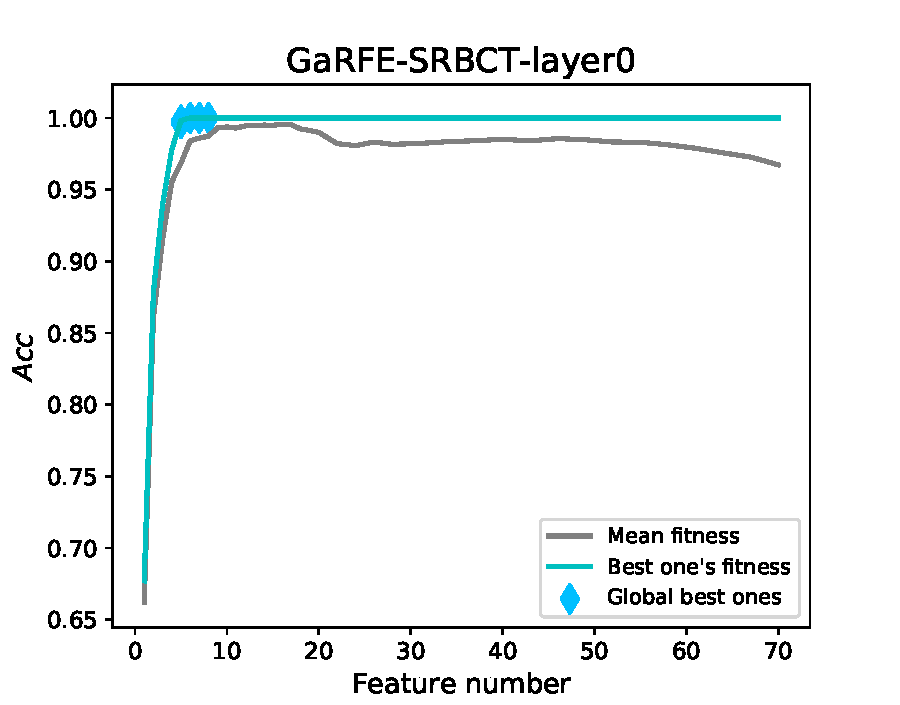
\includegraphics[height=1.65in]{pictures/SRBCT-RFE.pdf}
		\end{minipage}
		\begin{minipage}[t]{0.3\textwidth}
			\centering
			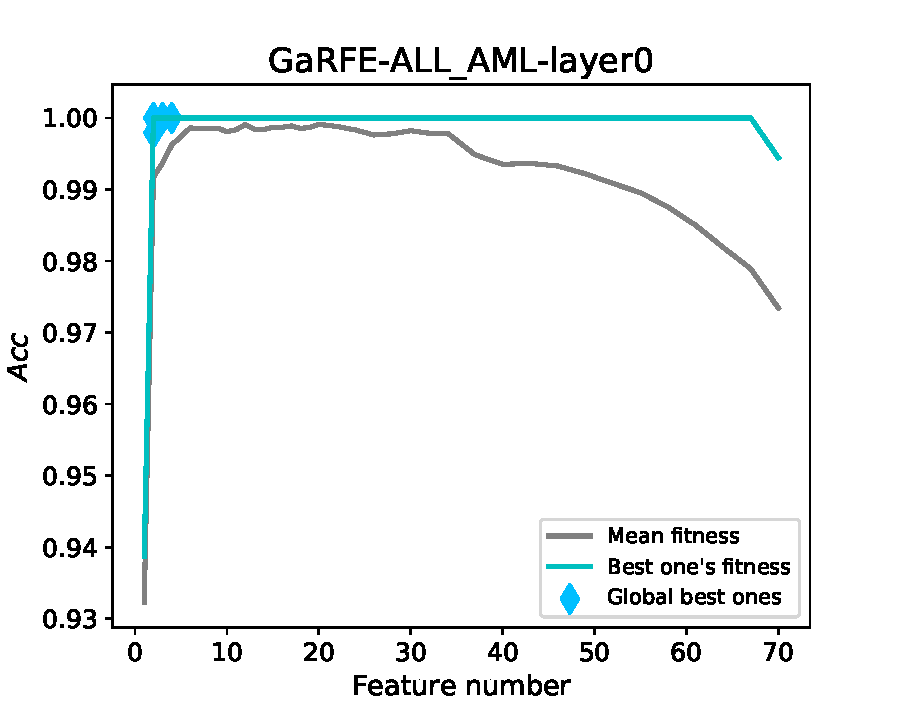
\includegraphics[height=1.65in]{pictures/ALLAML-RFE.pdf}
		\end{minipage}
		\begin{minipage}[t]{0.3\textwidth}
			\centering
			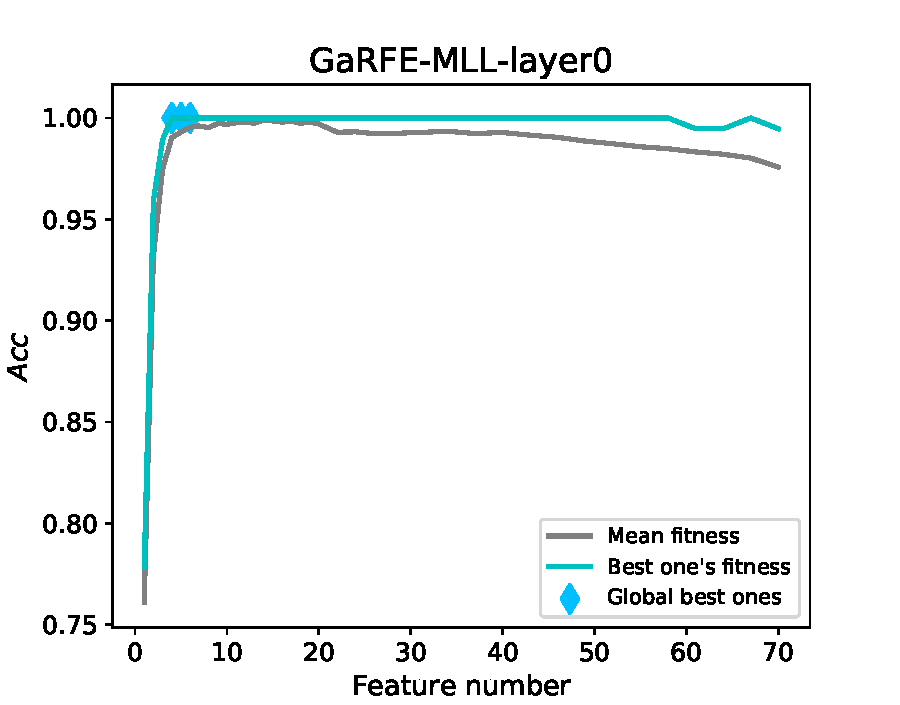
\includegraphics[height=1.65in]{pictures/MLL-RFE.pdf}
		\end{minipage}
		\caption{Three typical GaRFE processes on the three benchmark datasets from Dataset Two.}
		\label{Fig:3 RFE on benchmarks}
	\end{figure*}
	
	\begin{figure}[htbp]
		\centering
		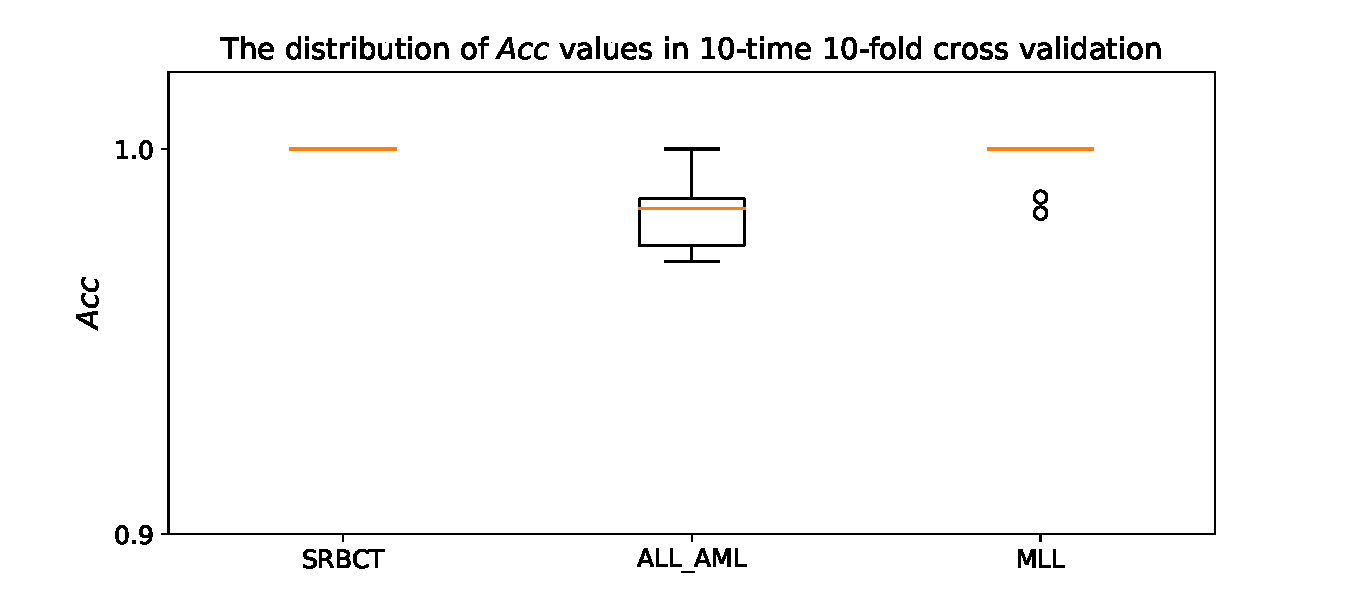
\includegraphics[width=0.47\textwidth]{pictures/CV2.pdf}
		\caption{The distribution of $Acc$ values in 10-time 10-fold CV for the selected gene combinations in Dataset Two.}
		\label{Fig:CV2}
	\end{figure}
	
	\subsection{Comparison with other methods on Dataset Two}
	
	The performance comparison based on \(Acc\) and the gene number with other state-of-the-art algorithms of feature selection on the three benchmark datasets are presented in Tables \ref{Tab:SRBCT RST}, \ref{Tab:ALLAML RST}, and \ref{Tab:MLL RST}, respectively.
	
	For the SRBCT dataset, MGRFE selected five genes and achieved 100\% $Acc$ in both 5-fold and 10-time 10-fold CV. In our computational experiments, combinations of four genes can reach 100\% train and test $Acc$ in 5-fold CV, but these gene combinations did not show classification stability in 10-time 10-fold CV. On the SRBCT dataset, Khan \emph{et~al.} \cite{P13} have applied an artificial neural network (ANN) and selected 96 genes to achieve 100\% $Acc$. Tibshirani \emph{et~al.} \cite{P20} have used the nearest shrunken centroid-based method (NSC) and achieved 100\% $Acc$ by means of 43 genes. Fu and Fu-Liu \cite{P10} employed support vector machine (SVM)-RFE and achieved 100\% $Acc$ by means of 19 genes. Pal \emph{et~al.} \cite{P17} have applied feature selection multilayered perceptron (FSMLP) and non-Euclidean relational fuzzy c-means clustering (NERFCM) and found seven genes important for 100\% $Acc$. Mohamad \emph{et~al.} \cite{P16} carried out improved binary PSO, and six genes were selected. Kar \emph{et~al.} \cite{W15} applied PSO and KNN and six genes were selected too. Moosa \emph{et~al.} \cite{P32} have achieved 100\% $Acc$ with the modified artificial bee colony algorithm (ABC) by means of five genes. Sharma \emph{et~al.} \cite{P18} have applied successive feature selection (SFS) with linear discriminant analysis (LDA) and nearest centroid classifier (NCC) and achieved 100\% train and test $Acc$ using four genes.
	
	\begin{table*}[!tp]
		\centering
		\caption{Performance comparison among the methods on the SRBCT dataset}
		
		\resizebox{0.9\textwidth}{!}{
		\begin{threeparttable}
		\label{Tab:SRBCT RST}
			\begin{tabular}{llllllllllll}
				\toprule
				Experiments & Methods & \multicolumn{4}{l}{Genes} & \multicolumn{4}{l}{CV $Acc$(\%)} & Train $Acc$(\%) & Test $Acc$(\%) \\
				\midrule
				Khan \emph{et~al.} (2001) \cite{P13} & ANN & \multicolumn{4}{l}{96} & \multicolumn{4}{l}{-} & 100 & 100 \\
				Tibshirani \emph{et~al.} (2002) \cite{P20} & NSC & \multicolumn{4}{l}{43} & \multicolumn{4}{l}{-} & 100 & 100 \\
				Fu and Fu-Liu (2005) \cite{P10} & SVM-RFE & \multicolumn{4}{l}{19} & \multicolumn{4}{l}{-} & 100 & 100 \\
				
				Yang \emph{et~al.} (2006) \cite{P22}				
				&& \multicolumn{2}{l}{5CV} & \multicolumn{2}{l}{LOOCV} & \multicolumn{2}{l}{5CV} & \multicolumn{2}{l}{LOOCV} & & \\		
				\cline{3-10}
				&& KNN & SVM & KNN & SVM & KNN & SVM & KNN & SVM & & \\
				\cline{3-10}
				& GS1 & 88 & 93 & 57 & 34 & 98 & 97.9 & 98.8 & 98.8 & {-} & {-} \\
				& GS2 & 90 & 99 & 77 & 96 & 98.1 & 99 & 98.8 & 100 & {-} & {-} \\
				& Cho's & 98 & 98 & 82 & 80 & 90.2 & 94.3 & 92.8 & 98.8 & {-} & {-} \\
				& F-test & 90 & 95 & 89 & 78 & 98 & 99.2 & 98.8 & 100 & {-} & {-} \\
				
				Pal \emph{et~al.} (2007) \cite{P17} & FSMLP+NERFCM & \multicolumn{4}{l}{7} & \multicolumn{4}{l}{-} & 100 & 100\\
				Li and Shu (2009) \cite{P15} & KLLE+LLE+PCA & \multicolumn{4}{l}{20} & \multicolumn{4}{l}{-} & 100 & 100\\
				
				Ji \emph{et~al.} (2011) \cite{P12} & PLSVIP & \multicolumn{4}{l}{24} & \multicolumn{4}{l}{-} & 100 & 100\\
				& PLSVEG & \multicolumn{4}{l}{15} & \multicolumn{4}{l}{-} & 100 & 100 \\
				Mohamad \emph{et~al.} (2011) \cite{P16} & IBPSO & \multicolumn{4}{l}{6} & \multicolumn{4}{l}{100} & {-} & {-} \\

				Zainuddin and Ong (2011) \cite{P23} & MSFCM+WNN & \multicolumn{4}{l}{10} & \multicolumn{4}{l}{10CV} & {-} & {-}\\
				\cline{7-7}
				\multicolumn{6}{l}{} & \multicolumn{4}{l}{100} & & \\

				Lee \emph{et~al.} (2011) \cite{P14} & AGA+KNN & \multicolumn{4}{l}{14} & \multicolumn{4}{l}{-} & 100 & 100\\
				Sharma \emph{et~al.} (2012) \cite{P18}
				& SFS+LDA with NCC & \multicolumn{4}{l}{4} & \multicolumn{4}{l}{-} & 100 & 100 \\
				& SFS+Bayes classifier & \multicolumn{4}{l}{4} & \multicolumn{4}{l}{-} & 100 & 90 \\
				& SFS+NNC & \multicolumn{4}{l}{4} & \multicolumn{4}{l}{-} & 100 & 95\\

				Chen \emph{et~al.} (2014) \cite{W5} & PSODT & \multicolumn{4}{l}{-} & \multicolumn{4}{l}{5CV} & {-} & {-} \\
				\cline{7-7}
				\multicolumn{6}{l}{} & \multicolumn{4}{l}{92.94} & & \\
				Kar \emph{et~al.} (2015) \cite{W15} & PSO+KNN & \multicolumn{4}{l}{6} & \multicolumn{4}{l}{98.0159} & 100 & 100\\
				Moosa \emph{et~al.} (2016) \cite{P32} & ABC & \multicolumn{4}{l}{5} & \multicolumn{4}{l}{-} & 100 & 100\\
				Dashtban and Balafar (2017) \cite{P33} & GA+SVM & \multicolumn{4}{l}{18} & \multicolumn{4}{l}{-} & 100 & 100\\
				
				\textbf{This paper} & \textbf{MGRFE} & \multicolumn{4}{l}{\textbf{5}} & \textbf{5CV} & \textbf{10-10CV} & \multicolumn{2}{l}{} & \textbf{100} & \textbf{100}\\
				\cline{7-8}
				\multicolumn{6}{l}{} & \textbf{100} & \textbf{100}\\
				\bottomrule
			\end{tabular}
	   		\begin{tablenotes}
	       % \tiny
		    \item In Tables \ref{Tab:SRBCT RST}, \ref{Tab:ALLAML RST}, and \ref{Tab:MLL RST}, 5CV means 5-fold cross validation; 10CV means 10-fold cross validation; 10-10CV represents 10-time 10-fold cross validation; and LOOCV represents leave one out cross validation.
	   		\end{tablenotes}
	   	\end{threeparttable}}
	\end{table*}
	
	For the ALL\_AML dataset, MGRFE selected two genes and achieved 100\% 5-fold $Acc$ and 98.2\% 10-time 10-fold CV $Acc$. On this dataset, Fu and Fu-Liu \cite{P10} have achieved 100\% train $Acc$ by means of 19 genes via SVM-RFE. Yang \emph{et~al.} \cite{P22} have employed a gene-scoring technique and SVM, and four genes were selected to achieve 98.6\% $Acc$ in leave one out cross-validation (LOOCV). Mohamad \emph{et~al.} \cite{P16} have selected two genes to reach 100\% CV $Acc$ based on improved binary PSO. Dashtban and Balafar \cite{P33} have applied integer-encoding GA and SVM and selected 15 genes with 100\% $Acc$. Ge \emph{et~al.} \cite{W16} have designed a two-step MIC-based method, and two genes were selected to reach 100\% $Acc$.
	
	For the MLL dataset, MGRFE selected three genes and achieved 100\% 5-fold $Acc$ and 99.7\% $Acc$ for 10-time 10-fold CV. On this dataset, Sharma \emph{et~al.} \cite{P18} have selected four genes with 100\% train and test $Acc$ based on SFS, LDA, and NCC. Mohamad \emph{et~al.} \cite{P16} have selected four genes with 100\% CV $Acc$ based on improved binary PSO. Dashtban and Balafar \cite{P33} have applied integer-encoding GA and SVM and selected 15 genes with 100\% $Acc$. Kar \emph{et~al.} \cite{W15} have employed PSO and KNN to select four genes with 100\% train and test $Acc$ and 92.5\% CV $Acc$.

	\begin{table*}[htbp]
		\centering
		\caption{Performance comparison among the methods on the ALL\_AML (Leukaemia) dataset}
		\label{Tab:ALLAML RST}
		\resizebox{0.9\textwidth}{!}{
			\begin{tabular}{llllllllllll}
				\toprule
				Experiments & Methods & \multicolumn{4}{l}{Genes} & \multicolumn{4}{l}{CV $Acc$(\%)} & Train $Acc$(\%) & Test $Acc$(\%) \\
				\midrule
				Fu and Fu-Liu (2005) \cite{P10} & SVM-RFE & \multicolumn{4}{l}{4} & \multicolumn{4}{l}{-} & 100 & 97.06 \\
				
				Yang \emph{et~al.} (2006) \cite{P22}
				&& \multicolumn{2}{l}{5CV} & \multicolumn{2}{l}{LOOCV} & \multicolumn{2}{l}{5CV} & \multicolumn{2}{l}{LOOCV} & & \\
				\cline{3-10}
				&& KNN & SVM & KNN & SVM & KNN & SVM & KNN & SVM & & \\
				\cline{3-10}
				& GS1 & 100 & 93 & 60 & 4 & 97.9 & 97.9 & 98.6 & 98.6 & {-} & {-}\\
				& GS2 & 85 & 98 & 10 & 25 & 97.1 & 97.4 & 98.6 & 98.6 & {-} & {-}\\
				& Cho's & 100 & 98 & 9 & 80 & 96.8 & 97 & 97.2 & 98.6 & {-} & {-}\\
				& F-test & 96 & 99 & 25 & 33 & 97.4 & 97.5 & 98.6 & 98.6 & {-} & {-}\\
				
				Shen \emph{et~al.} (2008) \cite{P19}
				& Stepwise & \multicolumn{4}{l}{3} & \multicolumn{4}{l}{-} & 90.83 & 88.14 \\
				& Pure TS & \multicolumn{4}{l}{5} & \multicolumn{4}{l}{-} & 95.83 & 94.24 \\
				& Pure PSO & \multicolumn{4}{l}{7} & \multicolumn{4}{l}{-} & 94.75 & 94.19 \\
				& HPSOTS & \multicolumn{4}{l}{7} & \multicolumn{4}{l}{-} & 98.08 & 95.81 \\
				Wong and Liu (2010) \cite{P21}
				& Probabilistic mechanism & \multicolumn{4}{l}{-} & SVM & KNN & & & {-} & {-}\\
				\cline{7-8}
				\multicolumn{6}{l}{} & 97.38 & 98.21 && & & \\

				Ji \emph{et~al.} (2011) \cite{P12}
				& PLSVIP & \multicolumn{4}{l}{9} & \multicolumn{4}{l}{-} & 100 & 100\\
				& PLSVEG & \multicolumn{4}{l}{8} & \multicolumn{4}{l}{-} & 100 & 100 \\
				
				Mohamad \emph{et~al.} (2011) \cite{P16} & IBPSO & \multicolumn{4}{l}{2} & \multicolumn{4}{l}{100} & {-} & {-} \\
				Zainuddin and Ong (2011) \cite{P23}
				& MSFCM+WNN & \multicolumn{4}{l}{10} & \multicolumn{4}{l}{10CV} & {-} & {-} \\
				\cline{7-7}
				\multicolumn{6}{l}{} & \multicolumn{4}{l}{98.61} & & \\

				Chandra and Gupta (2011) \cite{P9} & RNBC & \multicolumn{4}{l}{-} & 10CV & & & & {-} & {-} \\
				\cline{7-9}
				\multicolumn{6}{l}{} & RNBC & NBC & KNN \\
				\cline{7-9}
				\multicolumn{6}{l}{} & 94.29 & 84.29 & 85.71 & & & \\
				Kumar \emph{et~al.} (2012) \cite{P11} & GSA & \multicolumn{4}{l}{10} & \multicolumn{4}{l}{100} & {-} & {-}\\
				Kar \emph{et~al.} (2015) \cite{W15} & PSO+KNN & \multicolumn{4}{l}{3} & \multicolumn{4}{l}{95.8868} & 100 & 97.0588\\
				Ge \emph{et~al.} (2016) \cite{W16} & McTwo & \multicolumn{4}{l}{2} & \multicolumn{4}{l}{-} & 100 & 100\\
				Dashtban and Balafar (2017) \cite{P33} & GA+SVM & \multicolumn{4}{l}{15} & \multicolumn{4}{l}{-} & 100 & 100\\
				
				\textbf{This paper} & \textbf{MGRFE} & \multicolumn{4}{l}{\textbf{2}} & \textbf{5CV} & \textbf{10-10CV} & \multicolumn{2}{l}{} & \textbf{100} & \textbf{100}\\
				\cline{7-8}
				\multicolumn{6}{l}{} & \textbf{100} & \textbf{98.2}\\
				
				\bottomrule
		\end{tabular}}
	\end{table*}
	
	\begin{table*}[htbp]
		\centering
		\caption{Performance comparison among the methods on the MLL dataset}
		\label{Tab:MLL RST}
		\resizebox{0.9\textwidth}{!}{
			\begin{tabular}{lllllllllllll}
				\toprule
				Experiments & Methods & \multicolumn{4}{l}{Genes} & \multicolumn{4}{l}{CV $Acc$(\%)} & Train $Acc$(\%) & Test $Acc$(\%) \\
				\midrule
				
				Yang \emph{et~al.} (2006) \cite{P22}
				& & \multicolumn{2}{l}{5CV} & \multicolumn{2}{l}{LOOCV} & \multicolumn{2}{l}{5CV} & \multicolumn{2}{l}{LOOCV} & & \\
				\cline{3-10}
				& & KNN & SVM & KNN & SVM & KNN & SVM & KNN & SVM & & \\
				\cline{3-10}
				& GS1 & 29 & 99 & 97 & 56 & 94.8 & 95.2 & 97.2 & 97.2 & {-} & {-}\\
				& GS2 & 91 & 87 & 90 & 91 & 94.9 & 94.7 & 97.2 & 97.2 & {-} & {-}\\
				& Cho's & 93 & 89 & 23 & 44 & 96 & 95.5 & 97.2 & 95.8 & {-} & {-}\\
				& F-test & 99 & 100 & 65 & 31 & 95.4 & 94.8 & 95.8 & 95.8 & {-} & {-}\\
				
				Mohamad \emph{et~al.} (2011) \cite{P16} & IBPSO & \multicolumn{4}{l}{4} & \multicolumn{4}{l}{100} & {-} & {-} \\
				Chandra and Gupta (2011) \cite{P9} & RNBC & \multicolumn{4}{l}{-} & 10CV & &  & & {-} & {-} \\
				\cline{7-9}
				\multicolumn{5}{l}{} & & RNBC & NBC & KNN \\
				\cline{7-9}
				\multicolumn{5}{l}{} & & 87.14 & 80 & 68.57 & & & \\
				Sharma \emph{et~al.} (2012) \cite{P18}
				& SFS+LDA with NCC & \multicolumn{4}{l}{4} & \multicolumn{4}{l}{-} & 100 & 100 \\
				& SFS+Bayes classifier & \multicolumn{4}{l}{4} & \multicolumn{4}{l}{-} & 100 & 100 \\
				& SFS+NNC & \multicolumn{4}{l}{4} & \multicolumn{4}{l}{-} & 100 & 93 \\
				Chen \emph{et~al.} (2014) \cite{W5} & PSODT & \multicolumn{4}{l}{-} & \multicolumn{4}{l}{5CV} & {-} & {-}\\
				\cline{7-7}
				\multicolumn{5}{l}{} & & \multicolumn{4}{l}{100} & & \\
				Kar \emph{et~al.} (2015) \cite{W15} & PSO+KNN & \multicolumn{4}{l}{4} & \multicolumn{4}{l}{92.5439} & 100 & 100\\

				\textbf{This paper} & \textbf{MGRFE} & \multicolumn{4}{l}{\textbf{3}} & \textbf{5CV} & \textbf{10-10CV} & \multicolumn{2}{l}{} & \textbf{100} & \textbf{100}\\
				\cline{7-8}
				\multicolumn{6}{l}{} & \textbf{100} & \textbf{99.7}\\				
				
				\bottomrule
		\end{tabular}}
	\end{table*}
	
	\begin{table*}[htbp]
		\centering
		\caption{Literature mining in PubMed for the selected genes on Leukaemia, ALL1 and Gastric datasets}
		\resizebox{0.9\textwidth}{!}{
			\begin{threeparttable}
				\label{Tab:mining}
				\begin{tabular}{lllp{8em}p{13em}p{14em}}
					\toprule
					Dataset & Probe ID & Gene & PubMed hits for gene of interest & PubMed hits for gene of interest and leukemia\tnote{1} (\tnote{*}~Ratio1) &\\
					\midrule
					Leukaemia & \textit{M23197\_at} & CD33 Molecule(\textit{CD33}) & 3001 & 1753(58.41\%) &\\
					& \textit{M31523\_at} & Transcription Factor 3(\textit{TCF3}) & 569 & 115(20.21\%) &\\
					\midrule
					ALL1 & \textit{38319\_at} & CD3d molecule(\textit{CD3D}) & 84 & 13(15.48\%) &\\
					\toprule
					Dataset & Probe ID & Gene & PubMed hits for gene of interest & PubMed hits for gene of interest and cancer\tnote{2} (\tnote{**}~~Ratio2) & PubMed hits for gene of interest and gastric cancer\tnote{3} (\tnote{***}~~~Ratio3)\\
					\midrule
					Gastric & \textit{226237\_at} & collagen type VIII alpha 1 chain(\textit{COL8A1}) & 66 & 15(22.73\%) & 2(13.33\%)\\
					& \textit{226492\_at} & semaphorin 6D(\textit{SEMA6D}) & 41 & 13(31.71\%) & 1(7.69\%)\\
					& \textit{227771\_at} & leukemia inhibitory factor receptor alpha(\textit{LIFR}) & 463 & 159(34.34\%) & 2(1.26\%)\\
					\bottomrule
				\end{tabular}
				\begin{tablenotes}\scriptsize
					\item[1] gene of interest [All Fields] AND (``leukemia''[All Fields]).
					\item[2] gene of interest [All Fields] AND (``tumour''[All Fields] OR ``neoplasms''[MeSH Terms] OR ``neoplasms''[All Fields] OR ``tumor''[All Fields] OR ``cancer''[All Fields] OR ``carcinoma''[All Fields]).
					\item[3] gene of interest [All Fields] AND (``stomach''[All Fields] OR ``gastric''[All Fields]) AND (``tumour''[All Fields] OR ``neoplasms''[MeSH Terms] OR ``neoplasms''[All Fields] OR ``tumor''[All Fields] OR ``cancer''[All Fields] OR ``tumor''[All Fields] OR ``carcinoma''[All Fields]).
					\item[*] Ratio1 = \#(gene of interest-leukemia related literatures)$\big/$\#(gene of interest literatures).
					\item[**] Ratio2 = \#(gene of interest-cancer related literatures)$\big/$\#(gene of interest literatures).
					\item[***] Ratio3 = \#(gene of interest-gastric cancer related literatures)$\big/$\#(gene of interest-cancer related literatures)
				\end{tablenotes}
		\end{threeparttable}}
	\end{table*}




	\subsection{Biological inferences of the genes selected by MGRFE}
	
	The genes selected by MGRFE also have close relevance to the phenotypes in gene expression datasets. The genes selected by MGRFE with the 100\% 5-fold CV $Acc$ on datasets Leuk, Gas, and ALL1 are only two genes, three genes, and one gene, respectively.
	For each gene selected by MGRFE on these three datasets, we surveyed the number of published literatures involving the gene of interest and the related cancer phenotype in PubMed on 9th July, 2018. The literature-mining results on these three datasets are shown in Table \ref{Tab:mining}. Moreover, the gene probes finally selected by MGRFE on all 19 datasets are provided in the "S5" section of the Supplementary Material.
	In the Leukaemia dataset, our selected genes are \textit{CD33} and \textit{TCF3}. In PubMed, there are 3001 published literatures about \textit{CD33}, among which 1753 (58.94\%) papers discuss the relevance of \textit{CD33} to leukemia. And there are 569 publications about \textit{TCF3} in PubMed, among which 115 (20.21\%) papers confirming the association between \textit{TCF3} and leukemia. According to GeneCards, the E protein encoded by \textit{TCF3} performs a critical function in lymphopoiesis and is necessary for B and T lymphocytes. This gene is related to cancers including ALL (t(1;19), with \textit{PBX1}), childhood leukemia (t(19;19), with \textit{TFPT}), and acute leukemia (t(12;19)). In the Gastric dataset, genes \textit{COL8A1}, \textit{SEMA6D}, and \textit{LIFR} are selected by MGRFE, and there are 187 publications in PubMed confirming their relevance to cancer, but only five papers reveal their relations with gastric cancer. According to the excellent classification performance of these three genes on gastric cancer, they could be novel biomarker candidates for gastric cancer. In the ALL1 dataset, only one gene, \textit{CD3D}, is selected by MGRFE. There are 84 publications in PubMed about \textit{CD3D}, among which 13 (15.48\%) papers revealing the relevance of \textit{CD3D} to leukemia. In ref. \cite{Y34}, it has also been pointed out that gene \textit{CD3D} is one ideally discriminatory feature and gave a diagnostic rule when the expression of \textit{CD3D} is below a certain cutoff limit. Regarding \textit{CD3D}, GeneCards explains that this gene is involved in T-cell development and signal transduction, whereas defects in this gene will lead to severe combined immunodeficiency.

	\section{Discussion}
	
	The proposed MGRFE is a novel multilayer recursive feature elimination algorithm based on an embedded integer-coded genetic algorithm with a dynamic-length chromosome. MGRFE is aimed at selecting minimal discriminatory gene features associated closely with a phenotype. 
	MGRFE is designed as a complementary feature selection algorithm for high-dimensional data especially for gene expression data analysis. 
	Through the comprehensive comparison on 19 benchmark datasets with other state-of-the-art algorithms, MGRFE can  be successfully applied to cancer diagnosis and further biomedical research.
	
	The main innovation of MGRFE is an effective combination of the advantages of evolution calculation of the embedded GA with an explicit feature reduction of the RFE process in the basic feature search unit GaRFE. Therefore, our developed MGRFE can perform explicit feature elimination along with the evolution optimization search and achieve quick convergence speed.
	First, compared with other evolutionary-computation-based feature selection algorithms, our proposed MGRFE has shown higher convergence speed and obtained a slightly smaller discriminatory gene subset. For selecting informative gene features in a microarray, the state-of-the-art methods are commonly evolutionary-computation based. Meanwhile, almost all the existing evolution-based gene selection methods mainly rely on binary encoding and none of them take advantage of the RFE technique \cite{RN435,P33,RN437,W15,P32,RN438,RN416}. Nonetheless, the binary encoding has the shortcomings of the probable existing irrelevant features in a selected feature subset and high time cost to converge because there are thousands of genes in a microarray. Meanwhile, the fixed coding length of binary encoding leads to impossibility of explicit recursive feature reduction. Instead, MGRFE utilizes a variable-length integer-encoding technique in embedded GA and cuts down the encoding length recursively in an RFE process, which can quickly remove the irrelevant and redundant features and converge to a minimal informative feature combination. In 2017, Dashtban and Balafar also proposed an integer-coded GA with dynamic coding length for gene selection \cite{P33}, but they did not employ the recursive feature reduction technique. In fact, their method selected 18 and 15 genes with $Acc$ 100\% on the SRBCT and ALL\_AML datasets, respectively. But MGRFE only needs five and two genes to accomplish the same performance. 
	Second, compared with the original SVM-RFE \cite{P1}, MGRFE has better performance. SVM-RFE ranks all gene features by the weight vector from SVM with a linear kernel and removes the features with the smallest weights recursively. Nonetheless, SVM-RFE has the following three limitations: 1) The weight ranking can not completely reflect gene importance levels; 2) the top-ranked genes do not always form the optimal gene subset; 3) when a gene is removed, it has no opportunity to appear again. By contrast, the RFE process in MGRFE does not rank genes but introduces a random strategy to randomly discard the same number of genes in each individual between two GA runs, and when a gene is removed from an individual, it can still be present in other individuals. This arrangement leads to greater tolerance and stability. Besides, MGRFE selects gene combinations based on the sorting rule of a GA individual rather than selecting a gene individually, which has an advantage in finding the optimal gene subset. In 2005, Fu and Fu-Liu evaluated SVM-RFE on datasets SRBCT and ALL\_AML and finally selected 19 and four genes to achieve 100\% and 97.6\% test $Acc$s, respectively \cite{P10}. But MGRFE selected only five and two genes to attain 100\% $Acc$s in 5-fold CV for the same datasets.
	As for the selection operator of our embedded GA, the widely used roulette wheel selection \cite{P37} is inferior to our currently implemented truncation selection technique in this gene selection problem. The fitness gaps between different GA individuals are usually slight and account for only a tiny proportion of a fitness value. This situation provides all individuals with nearly the same area occupation in the roulette wheel and leads to the inefficiency of roulette wheel selection. 
	
	The 19 popular benchmark microarray datasets including multiclass and imbalanced datasets are employed to validate MGRFE. According to the performance comparison with other algorithms from 20 other studies, our proposed MGRFE is proved to be superior to most of the current state-of-the-art feature selection methods. MGRFE offers smaller informative gene subsets but the same or higher phenotype diagnosis accuracies. Many promising results are obtained by MGRFE on these datasets. MGRFE can reach $Acc$ 100\% within only five genes for 10 (52.6\%) of 19 datasets, and $Acc$ higher than 90\% within 10 genes for all 19 datasets, in 5-fold CV. MGRFE also possesses strong robustness for multiclass datasets and imbalanced datasets according to metrics $Sn$, $Sp$, $Avc$, $MCC$, and $AUC$.
	
	To conclude, the chief research contribution in theory is providing a novel feature selection method which combines embedded genetic algorithm with recursive feature elimination process, working as a creative thought for future research. To the best of our knowledge, none previous studies have designed an evolutionary algorithm using variable length integer encoding approach in a recursive manner to deal with the problem of minimal discriminatory feature selection in high-dimension datasets, which is described in this paper. Meanwhile, through theoretical and experimental comparisons, our proposed MGRFE could outperform mostly other state-of-the-art algorithms for gene selection on microarray data. Therefore, the proposed method MGRFE is worthy to be generalized to more feature selection problems on high-dimensional data characterized by the ”large \textit{p} small \textit{n}” paradigm and applied in several practical fields.

	Furthermore, our presented MGRFE would be useful in medical diagnosis as well as further biomedical research. The biological associations with phenotypes using literature mining in PubMed for the selected genes confirmed that the genes selected by MGRFE are biologically relevant to cancer phenotypes. Therefore, the informative genes selected by MGRFE could be novel biomarker candidates that are useful for better understanding the molecule mechanism related to the phenotypes and developing potential early detection and molecularly-targeted therapies for cancer diseases. Moreover, for clinical applications involving microarrays, MGRFE can contribute to the development of a potential simplified procedure for diagnosis of cancer subgroups by selecting the minimal discriminatory gene subsets, which will cut down the cost of medical diagnoses. 


\section*{Acknowledgments}

	The authors would like to thank the National Natural Science Foundation of China [Grant number 61472158, 71774154] and the Natural Science Foundation of Jilin Province (20180101331JC).
	Also, we are grateful to the two revered reviewers for their constructive comments.


\bibliographystyle{IEEEtran}
\bibliography{tcbb-bib}
	
\begin{IEEEbiography}[{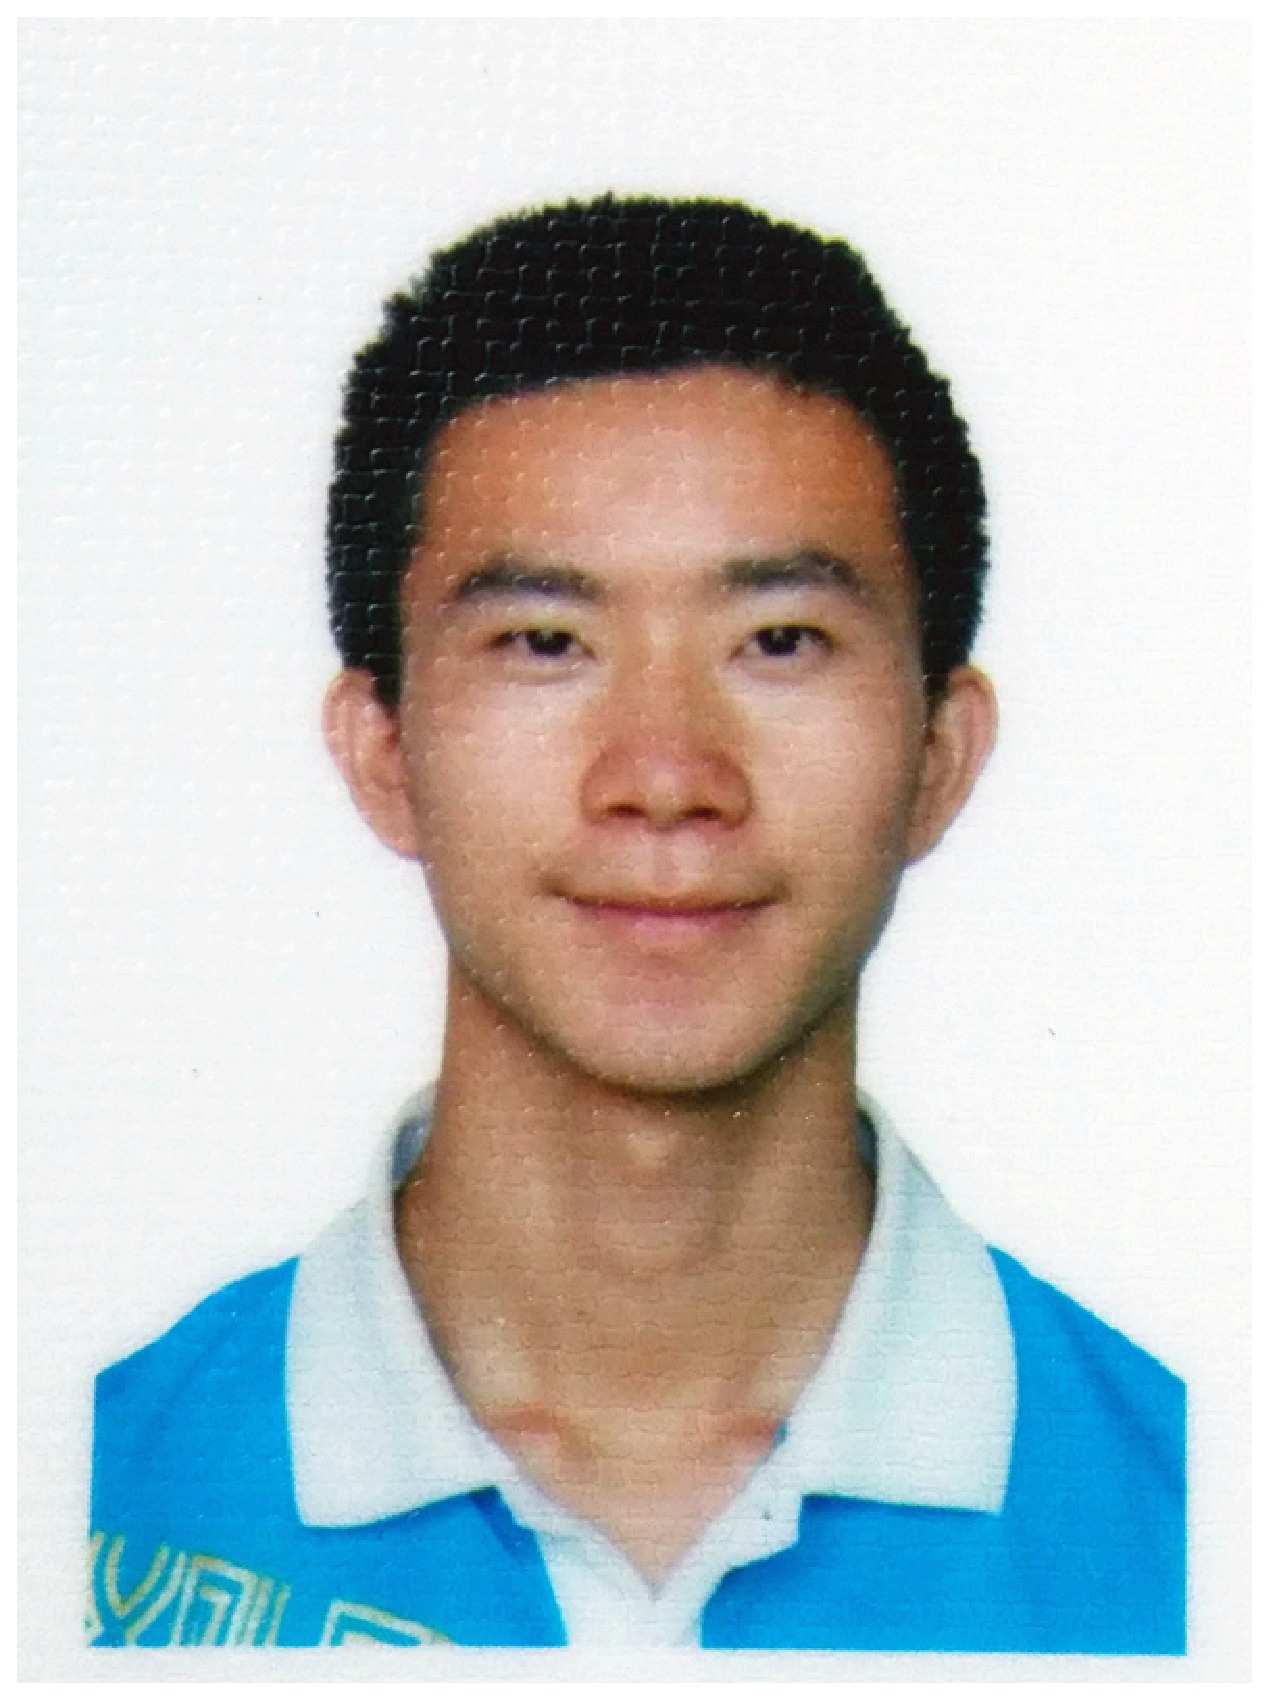
\includegraphics[width=1in,height=1.25in,clip,keepaspectratio]{pictures/CP-photo.eps}}]{Cheng Peng} 
	was born in Shanxi, China in 1996. He was a undergraduate in the College of Computer Science and Technology, Jilin University and received his BE degree in computer science and technology in 2018. His current research interests include machine learning and bioinformatics.
\end{IEEEbiography}

\begin{IEEEbiography}[{\includegraphics[width=1in,height=1.25in,clip,keepaspectratio]{pictures/YL-photo.eps}}]{Ying Li} 
	was born in Henan, China in 1978. She received the Ph.D. degree in computational mathematics from Jilin University, Changchun, China, in 2004. She is currently an associate professor with the College of Computer Science and Technology. She was a postdoctoral fellow at Tsinghua University from 2005 to 2007. She was a visiting scholar at University of Georgia of United Kingdom from 2011 to 2012. She has published more than 30 journal and conference papers. Her current research interests include machine learning and bioinformatics.
\end{IEEEbiography}
	
\end{document}

